\documentclass[a4paper]{article}
\usepackage{amsfonts}
\usepackage{amsmath}
\usepackage{amssymb}
\usepackage{graphicx}
\usepackage{extarrows}

\newcommand{\integral}{\displaystyle\int}
\newcommand{\limit}{\lim\limits}

\begin{document}

\noindent \large Auteur: Seda Jusjajeva\\
\noindent \large Studierichting: Informatica\\
\noindent \large Oefeningenreeks 5G nr. 1.1\\

\medskip

\normalsize



$f(x) = x^3$ \\

\begin{figure}[h]
\centering
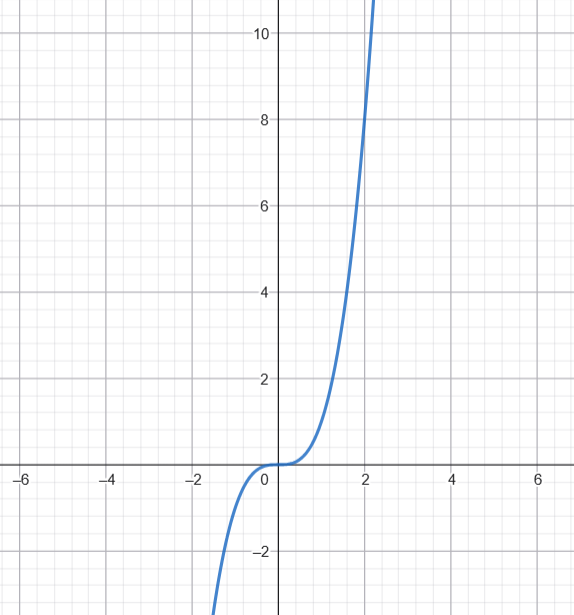
\includegraphics[width=8cm]{5G-1.1-seda.jusjajeva.INF.png}
\end{figure}

$V = \pi\integral_{0}^{2}\left(x^3\right)^2dx = \pi\integral_{0}^{2} x^6dx = \pi\left[\dfrac{x^7}{7}\right]_{0}^{2} = \pi\left(\dfrac{2^7}{7} - \dfrac{0^7}{7}\right) = \dfrac{128\pi}{7} $ \\




\begin{thebibliography}{999}
%\bibitem{a} Referentie
\end{thebibliography}
\end{document}